\documentclass[useAMS,usenatbib,referee]{biom}
%\usepackage{authblk}
\usepackage{graphicx}
%\usepackage{subcaption}
%\usepackage{float}
\usepackage{amsmath}
%\usepackage{bm}
%\usepackage[authoryear,round, longnamesfirst]{natbib}
%\usepackage{textcomp}
%\usepackage{setspace}
%\usepackage{appendix}
%\doublespacing
%\usepackage{fancyhdr}
\usepackage[]{todonotes}
%\presetkeys{todonotes}{fancyline, color=white}{}
\usepackage{url}

%\pagestyle{fancy}
%\rhead{That's not the Mona Lisa}
%\lhead{}

%\usepackage{geometry}
%\geometry{margin=4cm}

%\usepackage{lineno}
%\linenumbers
%\linespread{1.6}

\title[How to interpret SCR density surface estimates]{That's not the Mona Lisa! How to interpret spatial capture-recapture density surface estimates}

\author{Ian Durbach$^{1,2,*}$, Rishika Chopara$^{3}$, David L. Borchers$^{1,2}$, Rachel Phillip$^{1}$, Koustubh Sharma$^{4}$ \and Ben C. Stevenson$^{3}$ \\
$^{1}$Center for Research into Ecological and Environmental Modelling, \\ School of Mathematics and Statistics, Univeristy of St Andrews, Scotland \\
$^{2}$Center for Statistics in Ecology, the Environment and Conservation, \\ Department of Statistical Sciences, University of Cape Town, South Africa \\
$^{3}$Department of Statistics, University of Auckland, Auckland 1010, New Zealand \\
$^{4}$Snow Leopard Trust, Seattle, Washington, United States of America \\
\email{indurbach@gmail.com}}

\begin{document}

\begin{abstract}
Spatial capture-recapture methods are often used to estimate density surfaces, and these estimates are often misinterpreted. In particular, spatial change in density is confused with spatial change in uncertainty about density. We illustrate correct and incorrect inference visually by treating an image of the Mona Lisa as an activity center intensity or density surface and simulating spatial capture-recapture survey data from it. Inferences can be drawn about the intensity of the point process generating activity centers, and about a single realization of this process. We show that treating estimates of a realization of the process as estimates of the intensity of the process results in invalid and misleading ecological inferences, and that estimates of the realization are highly dependent on where the detectors are placed and how much survey effort is used. Estimates of the activity center density surface should be obtained by estimating the intensity of a point process model for activity centers. Practitioners should state explicitly whether they are estimating the intensity or the realization, and estimates of the realization should not be confused with estimates of the intensity.
\end{abstract}


\begin{keywords}
Density surface, point processes, spatial capture-recapture.
\end{keywords}

\maketitle 

\section{Introduction}

Spatial capture-recapture (SCR) models \citep*{Efford:04,Borchers+Efford:08, Royle+Young:08} are now widely used to estimate animal abundance and distribution from a variety of data types, including that from camera-traps, hair snares and scat surveys, live-captures, and acoustic detectors. These methods use the location of the detectors (e.g.\ traps) and the locations at which animals were detected (their spatial capture histories) to estimate animal density. The methods have two basic components: a spatial model that quantifies animal activity center (hereafter abbreviated to ``AC'') density at all points in the survey region, and an encounter model that quantifies the expected detection frequency or detection probability, given the AC locations and the detector locations. 

SCR density estimates are often presented graphically in the form of estimated density maps, these being easy to absorb and interpret, at least on the face of it.  However, there are various kinds of density maps that one can produce from SCR analyses and depending on what is presented, it is easy to misinterpret the maps. The most common form of misinterpretation is treating maps that include both spatially varying uncertainty about AC locations and spatially varying AC density estimates as if they were maps of AC density alone. There is also a lack of clarity about whether it is AC density or space use density that is being presented.

Examples include \cite{Dorazio+Karanth:17}, who say that such maps effectively provide  ``a species distribution model, even in cases where spatial covariates of abundance are unknown or unavailable'', \cite{Alexander+al:15}, who present a map (Figure 4) that include both spatially varying uncertainty about location and spatially varying AC density and refer to it as the ``spatial distribution of snow leopards'', and \cite{Elliot+Gopalaswamy:16}, who present the same kind of map (Figure 2) and refer to it as the ``pixel-specific lion density''. Minor variations on these themes can be found in many papers, for example ``spatial distribution of the Amur leopard density'' \citep{Qi2015}, ``a pixelated map showing fine-scale variation in density'' \citep{Fouche2020},``spatial variation in the location of estimated activity centers'' \citep{Blanc2013}, ``pixelated SPACECAP leopard density maps'' \citep{Devens2021}, ``pixel-specific densities of elephants'' \citep{Goswami2019}, ``a pixelated density map showing relative leopard density \citep{Kandel2020}, ``spatial density estimate of common leopards'' \citep{Goldberg2015}, ``density estimates in home-range centers (number of jaguars per 0.226km$^2$)'' \citep{Lavariega2020}, ``spatial patterns of dhole densities'' \citep{Srivathsa2021}, ``mean posterior density of Amur tiger'' \citep{Xiao2016}, and \cite{Chandler+Royle:13} who say ``Density surface maps can be produced by discretizing the state-space and tallying the number of activity centers occurring in each pixel during each MCMC iteration''.

The problems with interpretation of such maps arises because (a) there are various kinds of ``density'', (b) uncertainty about the locations of ACs varies spatially and this fact must be (but is often not) taken into account when interpreting estimated density surfaces from SCR surveys, and (c) there is a failure to clearly distinguish between AC density and usage density.

We start by describing different kinds of densities involved in SCR surveys, because in any discussion of density surfaces, we need to be clear about what ``density'' means. 

\section{Different kinds of density}\label{different-densities}

Let us assume that ACs are independently generated by a Poisson process over some region of interest $\mathcal{S}$. Such a process is fully characterized by its intensity function. We could assume that the process is homogeneous, which implies that ACs have independent uniform distributions on $\mathcal{S}$. Alternatively, we can use an inhomogeneous process based on spatially referenced covariates, where the intensity at location $\bm{s}$ is given by $D(\bm{s})=\exp\left\{\beta_0 + \sum_{k=1}^K\beta_kx_k(\bm{s})\right\}$. Here, $\bm{s} \in \mathcal{S}$, $x_k(\bm{s})$ is the $k$th of $K$ spatially referenced covariates evaluated at $\bm{s}$, $\beta_0$ is an intercept parameter, and $\beta_k$ is the slope parameter for the $k$th spatially-referenced covariate. We distinguish between two kinds of spatial ``density'' below. 

\subsection{Expected AC density surface} \label{s:eacd}

The first we call the ``expected AC density'' surface. This is $D(\bm{s})$, the intensity function of the underlying point process that is assumed to have generated the ACs. We use the term ``expected'', because the intensity of the point process at $\bm{s}$ is approximately the expected number of ACs per unit area generated by the process in some small region surrounding $\bm{s}$ (and is exactly the expectation as the area of the region approaches zero). This quantity depends only on the parameters of the point process, and is not specific to any particular realistion of points -- indeed it is an average over all possible realizations. The expected number of ACs generated by the process in any region can be calculated by integrating the intensity function over the region. For example, the expected number of activity centers in $\mathcal{S}$ is $\int_{\mathcal{S}} D(\bm{s}) \, d\bm{s}$. We can estimate the expected AC density surface by fitting a Poisson process model to our data, and plugging the resulting estimates of $\bm{\beta}$ into the intensity function. We denote this estimated surface as $\widehat{D}(\bm{s})$. 

Maximum likelihood and Bayesian SCR methods for estimating $\bm{\beta}$ and hence the expected AC density surface are documented in a good number of papers, starting with \cite{Borchers+Efford:08} and \cite{Royle+Young:08}. Both approaches are based on SCR likelihood functions that include a component specifying the AC density surface, which may depend on spatially-referenced covariates. 

\subsection{Realized AC density surface} \label{s:racd}
 
The second kind of density we call the ``realized AC density''. Suppose that we divide $\mathcal{S}$ into a grid of cells, the $j$th of which comprises the points in the set $\mathcal{C}_j$, and each has area $a$. Suppose also that we don't observe the ACs, but we treat them as random variables, each with its own distribution and we have a probability density function (PDF) for each AC: $f_1(\bm{s}),\ldots,f_N(\bm{s})$. We define random variables $\delta_{1j},\ldots,\delta_{N_j}$ ($j=1,\ldots,N$), such that the $\delta_{ij}=1$ if the $i$th AC is in $\mathcal{C}_j$ and $\delta_{ij}=0$ otherwise. The expected value of $\delta_{ij}$ is then $E_r(\delta_{ij})=\int_{\mathcal{C}_j} f_i(\bm{s}) \, d\bm{s}$, where integration is over the points in $\mathcal{C}_j$.

The expected value of $\delta_{\cdot j}=\sum_{i=1}^N\delta_{ij}$ is $\sum_{i=1}^N E_r(\delta_{ij})$. This can be interpreted as the expected number of ACs that are in cell $j$. With this interpretation, we define $D_{rj} = \sum_{i = 1}^N E_r(\delta_{ij})/a$ to be the ``realized AC density'' in cell $j$, and the limit of this function as $\mathcal{C}_j$ shrinks to the point $\bm{s}$, to be the realized AC density surface at $\bm{s}$:
\begin{equation}
D_r(\bm{s})=\sum_{i=1}^N f_i(\bm{s}) \label{eq:realized-D}
\end{equation}
\noindent
The realized AC density surface is a derived quantity, in the sense that it is a product of whatever underlying model is assumed to generate the $f_i(\bm{s})$. Given estimates for the number of ACs in the survey region, $\widehat{N}$ and the PDFs of their locations, $\widehat{f}_i(\bm{s}),\ldots,\widehat{f}_{\widehat{N}}(\bm{s})$, we can estimate the realized AC density surface as $\widehat{D}_r(\bm{s})=\sum_{i = 1}^{\widehat{N}}\widehat{f}_i(\bm{s})$, with estimates of the expected number and density of ACs in the $j$th cell as $\widehat{E}_r(\delta_{\cdot j})=\int_{\mathcal{C}_j}\widehat{D}_r(\bm{s}) \, d\bm{s}$ and $\widehat{D}_{rj}=\int_{\mathcal{C}_j}\widehat{D}_r(\bm{s})\, d\bm{s}/a$ respectively.

Again, maximum likelihood and Bayesian SCR methods for estimating the AC PDFs and hence the realized AC density surface are well documented, for example in Section 4.3 of \cite{Borchers+Efford:08} for maximum likelihood methods and the section ``Estimating derived parameters'' on page 3238 of \cite{Royle+al:09b} for Bayesian methods. The estimated AC PDF $\widehat{f}_i(\bm{s})$ is a probability density for the location of individual $i$'s AC, conditional on it's capture history and parameter estimates from a fitted SCR model ($f_i(\bm{s})$ can be thought of as the AC PDF that would be obtained with the true parameter values). Note that we can obtain AC PDFs for undetected animals because we know their capture histories -- namely no capture at every detector -- and these will be the same AC PDF unless there are individual-level covariates that affect detection probability estimates (a complication that we ignore). Separating out the estimated AC PDFs for $n$ detected animals, $\widehat{f}_i(\bm{s}),\ldots,\widehat{f}_n(\bm{s})$, from those for each of $\widehat{N}-n$ undetected individuals, $\widehat{f}_u(\bm{s})$, we obtain $\widehat{D}_r(\bm{s}) = \sum_{i = 1}^n \widehat{f}_i(\bm{s}) + (\widehat{N} - n)\widehat{f}_u(\bm{s})$. It is this surface, usually plotted after discretising the survey region into cells, that many publications (including those listed in the Introduction) interpret as a density surface for AC or animal locations. While perhaps done for brevity, referring to the realized AC density surface as an estimated density of {\it animals} (rather than ACs) makes the additional error of ignoring animal movement around ACs. An AC PDF captures only uncertainty about where the AC is located. It is not equivalent to an estimate of the animal's home range and does not provide meaningful information on animal space use --  animals may be present at locations with realized AC densities close to zero.

\begin{figure}[htbp]
\centering
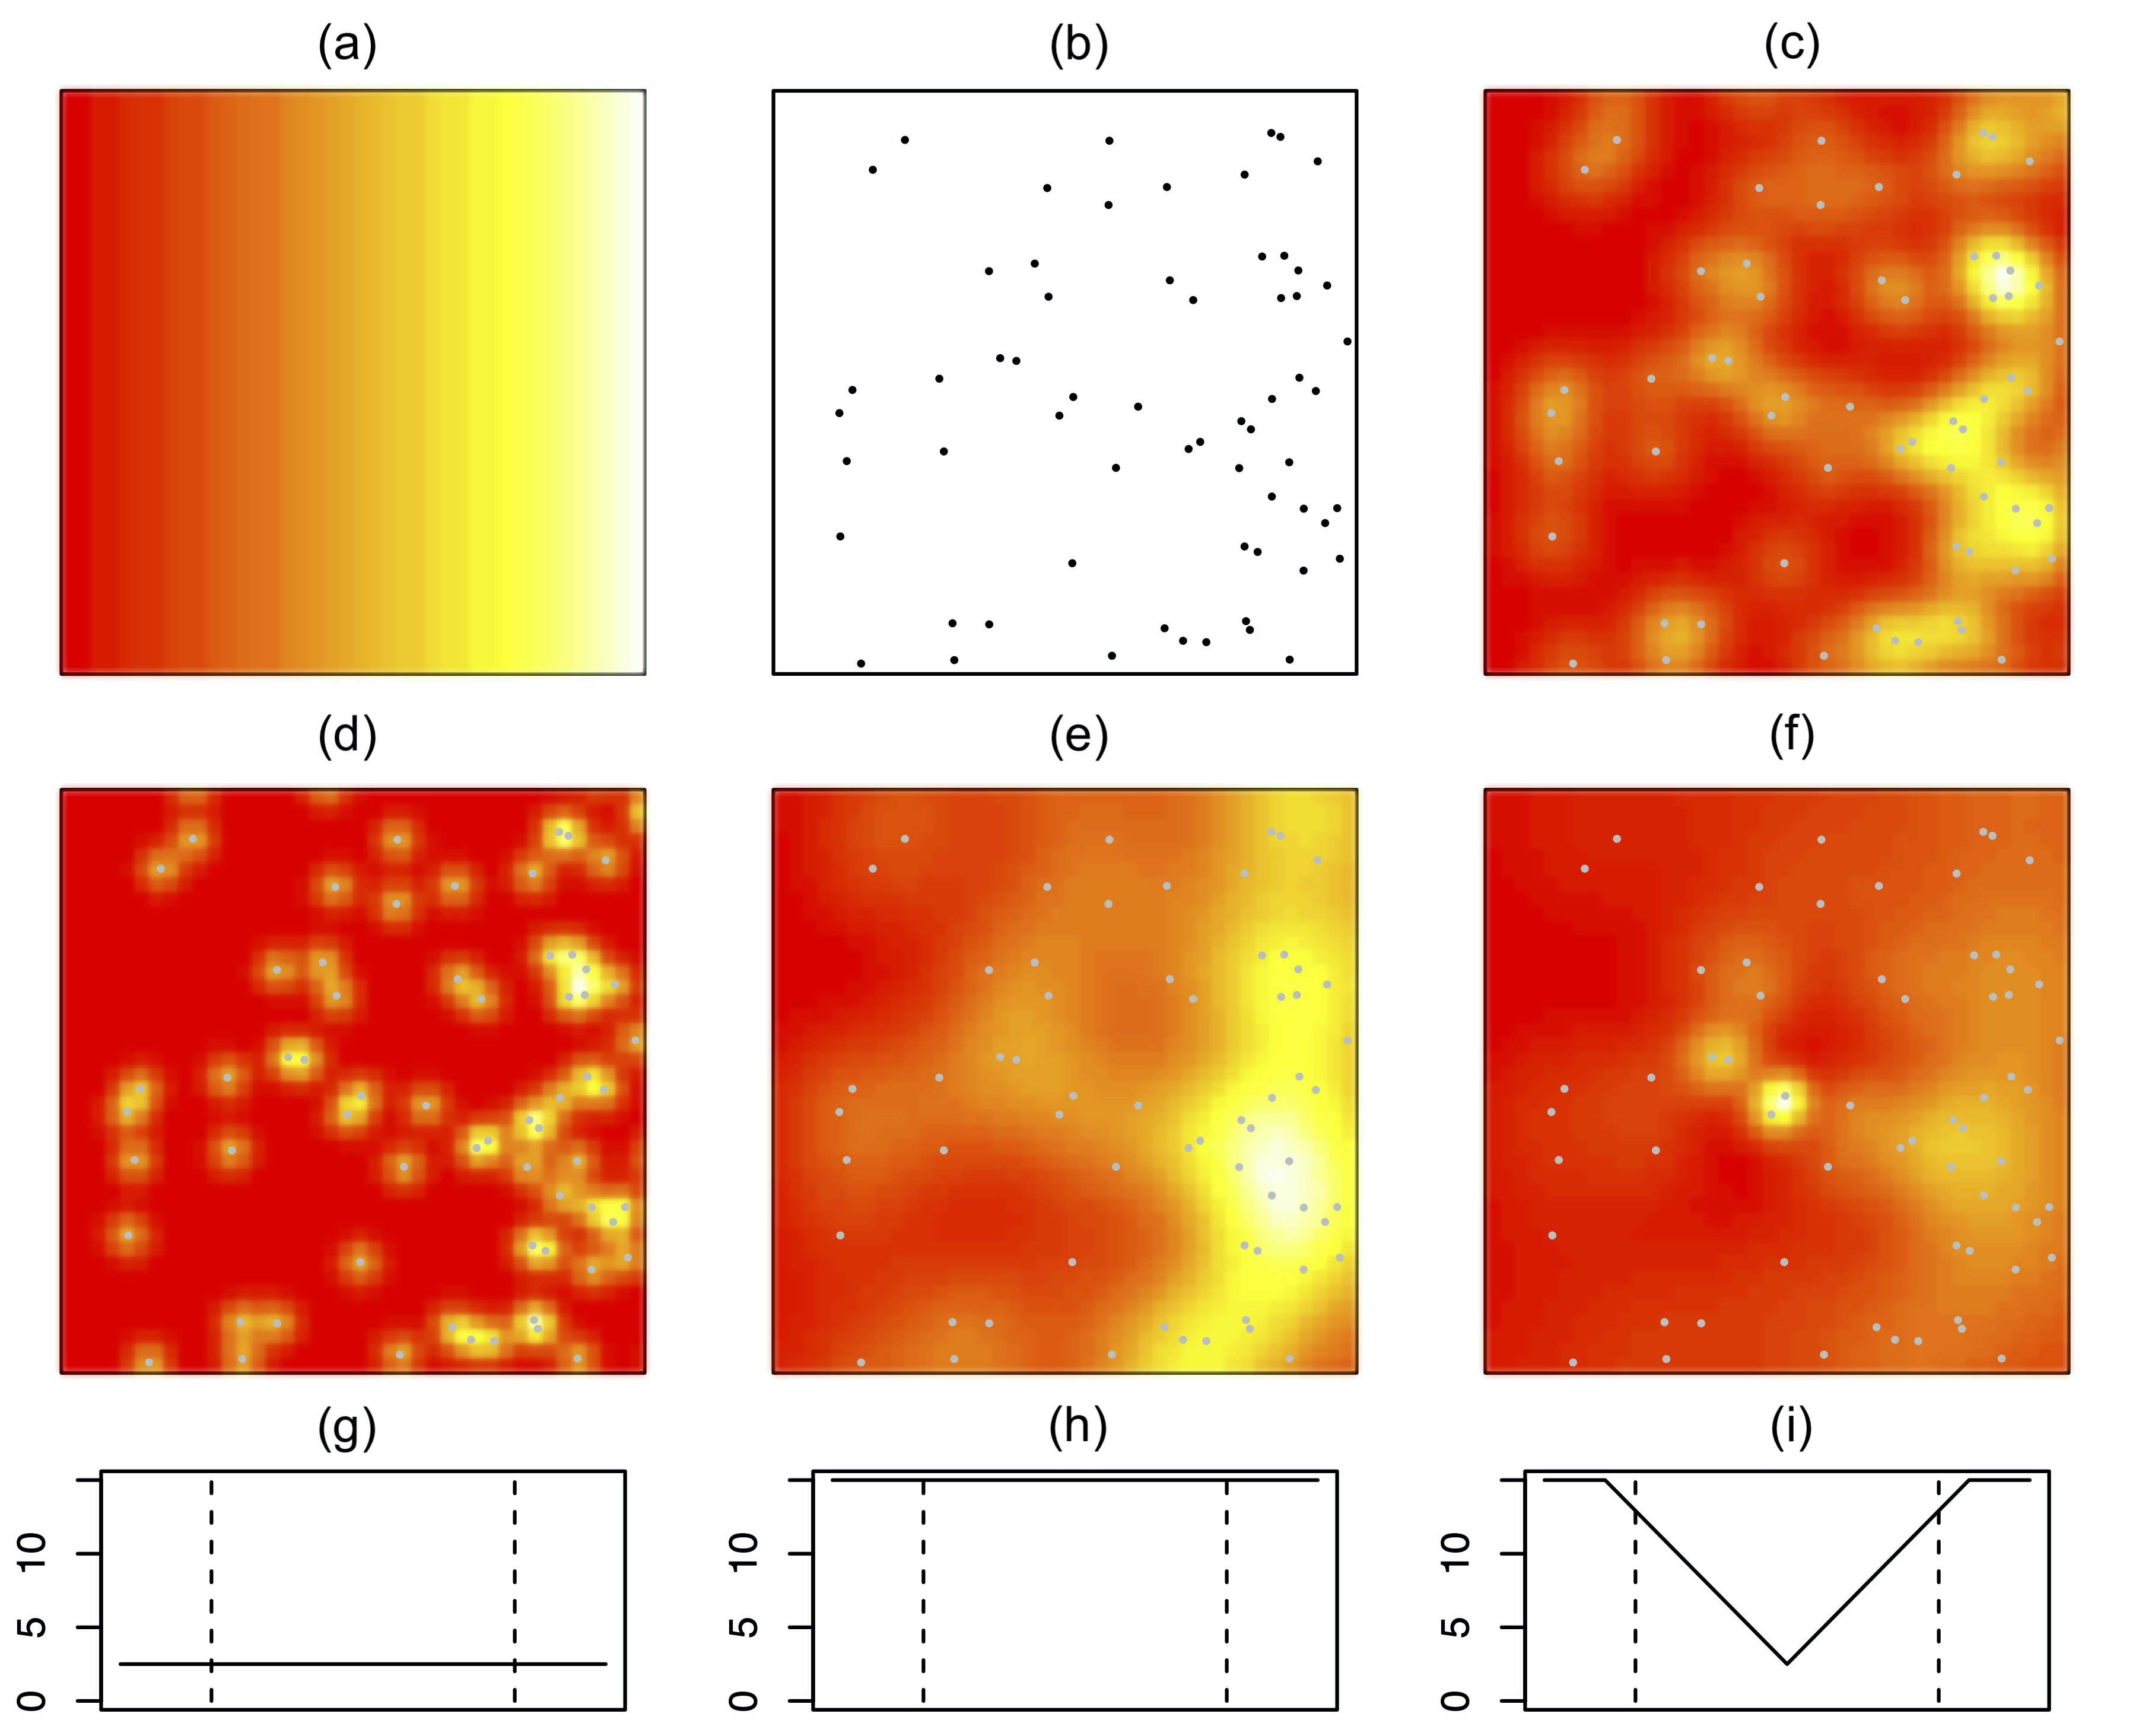
\includegraphics[width=\textwidth]{example-densities.jpg}
\caption{Examples of (a) an AC intensity (density) surface, (b) a realization of ACs from this intensity surface. Panels (c) to (d) show the realized AC density in (b), when the individual AC PDFs ($f_1(\bm{s}),\ldots,f_N(\bm{s})$) are bivariate normal with standard errors (c) $\sigma=2.5$, (d) $\sigma=15$, and (e) $\sigma=2.5$ for an AC at the center of the plot (dimension 100$\times100$), rising linearly to $\sigma=15$ by the edge of the plot. True ACs shown as grey dots. The color scales of panels (c) to (e) are such that the highest and lowest densities in each plot is the same. Panels (f) to (h) plot the standard errors of the AC PDFs in (c) to (e) against the x-axis. Vertical dashed lines show the extent of the survey region in panels (c) to (e); a buffer beyond this is included because points outside it affect the plot within the survey region. Color version of figures can be found in the electronic version of this article.}
\label{fig:densities}
\end{figure}

\subsection{Estimated density surfaces}
Figure~\ref{fig:densities} shows examples of both types of density, together with realized AC locations, for a simplified example in which we directly specify the AC PDFs, rather than having to estimate them, and assume that $N$ is known. This allows us to demonstrate our main points while avoiding some of the complexities of SCR surveys (these are addressed in later sections). 

If we are interested in explaining why density tends to be high in some places and lower in others, or in characterizing the process that governs the distribution of ACs, then we are primarily interested in estimating a density surface like that shown in Figure~\ref{fig:densities}(a). In this example, it is easting that influences this density, but in general it might be any of a wide variety of habitat or environmental covariates, some of which may be unobserved and evidenced only by spatial clustering of ACs. 

If we are interested only in where the ACs are, and not in explaining why they are there, then Figure~\ref{fig:densities}(b) suffices. But if we cannot observe ACs, as is typically the case, we need to model the PDFs of ACs and construct a density surface estimating Equation \eqref{eq:realized-D}. For example, Figure~\ref{fig:densities}(c)-(e) shows realized AC density surfaces when the individual AC PDFs are bivariate normal distributions with small variance in (c), larger variance in (d), and variance increasing linearly from the center of the plot in (e). The PDFs ``spread'' information about each AC's location according to a bivariate normal distribution, with greater spreading when there is greater uncertainty about location (greater variance).

Ignoring the actual AC dots (because they cannot be observed), Figure~\ref{fig:densities}(c) gives a reasonable visual representation of where the ACs are. It is much more difficult to pick out individual ACs from Figure~\ref{fig:densities}(d), but it gives a reasonable representation of where the high- and low-density regions of ACs are -- much like Figure~\ref{fig:densities}(a), but customized somewhat for this particular realization of AC locations rather than their long-run average locations. Note, however, that these two figures are representations of exactly the same set of ACs and that if one interprets them as plots of AC density, they contradict each other. Figure~\ref{fig:densities}(c) says that almost all the region has low density (red in the plot) and that there are lots of small high-density regions, while Figure~\ref{fig:densities}(d) says that there is much less variation in density, that there are large swathes of higher density (the yellow towards the right) and large swathes of low density towards the left. The reason that Figure~\ref{fig:densities}(d) shows less variation in density is not that there is less variation in the population (there are exactly the same ACs in both (c) and (d)), it is that we are less sure about the location of the ACs in (d). To interpret this as less variation in AC density is to invite incorrect ecological inferences.

Now what about Figure~\ref{fig:densities}(e)? If this is interpreted as indicating where the high and low-density regions are, it is misleading. It says that the highest density region is in the center of the plot, and that the region with most variation in density is the central region, which is not true. 

The fact that there is only small uncertainty about AC location in the center of the plot and large uncertainty error at the edges means that the ACs near the center are not ``spread'' much and therefore appear as higher peaks in the surface, with low regions where there are no ACs. Near the edges of the plot, on the other hand, uncertainty about AC location is high and ACs are ``spread'' a lot, which both flattens the peaks at individual AC locations and ``fills in'' the troughs where there are no ACs. 

It is a feature of SCR surveys that the AC locations of individuals farther from the detector array tend to be estimated with greater uncertainty than individuals within the array. This is illustrated in Figure~\ref{fig:screrr}, which shows the estimated probability density functions for ACs of two animals detected on a simulated SCR survey with a 4$\times$4 array placed in the center of the population shown in Figure~\ref{fig:densities}(b). The reason contours in the top right of the figure ``avoid'' the triangle is because the detection function range, estimated from the whole survey, not just the points shown, is large and if the AC was near the triangle, other detectors would have high probability of detecting it. The fact that they did not makes them ``repel'' the AC. 

\begin{figure}[htbp]
\centering
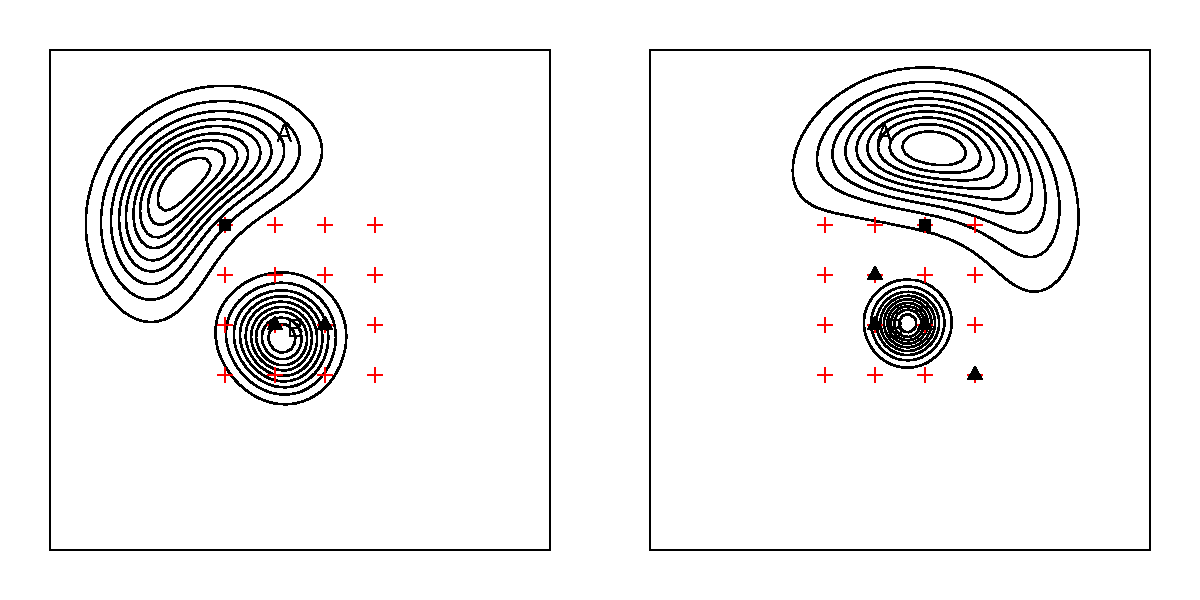
\includegraphics[width=0.5\textwidth]{screrr.pdf}
\caption{Estimated probability density function contours for two detections in an SCR survey of the population shown in Figure~\ref{fig:densities}(b). Detectors are shown as red crosses. The lower left individual was detected at detectors indicated by black squares, the upper right individual only by the top right detector indicated by a black triangle.}
\label{fig:screrr}
\end{figure}

\section{Methods}

We illustrate what each estimated surface gives the SCR practitioner, and which interpretations are valid and useful, by simulating data from a density surface that has an easy visual interpretation. To do this, we turned one of the most recognizable images in Western culture, the Mona Lisa, into a density surface. We created a greyscale version of a region of the original image (Figure \ref{mlinputs}a) in which values give the intensity of the point process generating ACs, and lighter areas correspond to higher densities. The intensity surface is continuous, with intensities defined at any point $\bm{s}$. Although any pixelated image must be discrete at some scale, the resolution we use in Figure \ref{mlinputs}(a) is sufficiently high (1200$\times$ 1200 pixels) to visually make the point that the surface is continuous.  

The image's pixel intensities can be arbitrarily scaled to integrate to the expected number of activity centers over the surface. We chose this to be 80, on the basis that this is sufficient to illustrate our main points and also broadly typical of many wildlife surveys. We then generated a single realization of points from this surface (from an inhomogeneous Poisson process with average intensity of 80), which resulted in 77 ACs being generated (Figure \ref{mlinputs}(b)).

\begin{figure}[htbp]
\centering
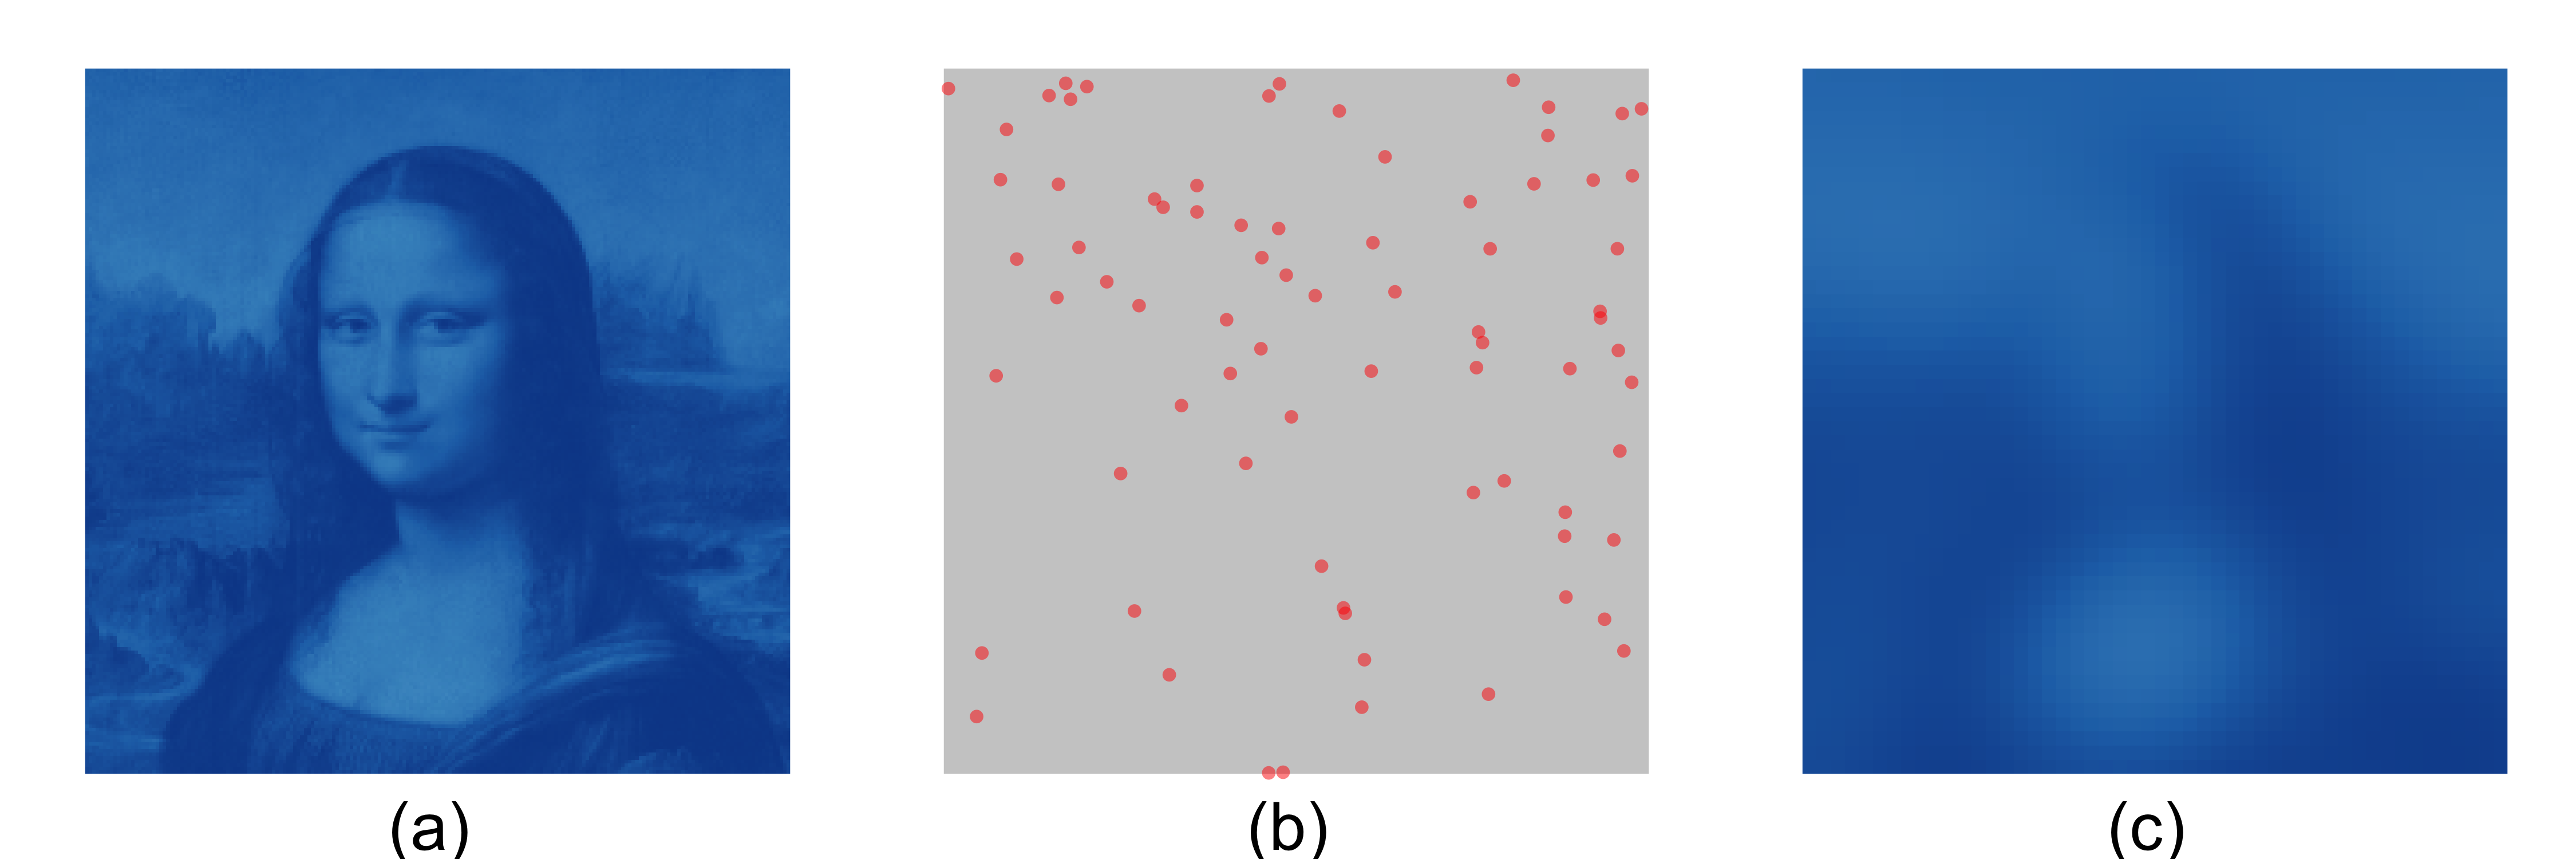
\includegraphics[width=1\textwidth]{mona_inputdata.png}
\caption{Input data for the Mona Lisa simulation study. Panel (a) shows a greyscale version of the Mona Lisa treated as an expected AC density surface. Panel (b) shows a single realization of 77 ACs generated from the surface in (a), while (c) shows a spatially-varying covariate that is correlated with true density, and which is used to estimate expected AC density surfaces.}
\label{mlinputs}
\end{figure}

We simulated capture histories from the population using a half-normal encounter rate function $\lambda(d) = \lambda_0\exp\{-d^2/(2\sigma^2)\}$, where $\sigma$ is a scale parameter determining how quickly the encounter rate decreases with $d$, the distance between the detector and the activity center, and $\lambda_0$ is the expected number of encounters at a detector that is at animal's AC ($d=0$). Arbitrarily defining the dimensions of the image to be $50\times 50$ units, we set $\sigma=4$ and used two different detector arrays: a $3\times3$ array centered at $x=18$ and $y=24$ (Figure~\ref{mona3x3}), and a $7\times 7$ array covering the entire image (Figure~\ref{mona7x7}). Note that the survey region is closed, in the sense that there are no detectable ACs beyond its borders. Both arrays had a fixed spacing of $2\sigma=8$ between detectors. The number of simulated detections at each detector were Poisson random variables with expected values equal to the encounter rate function evaluated at the distances of detectors from ACs. In order to illustrate how realized and expected AC density surfaces change with increasing sample sizes, we simulated capture histories with three different survey effort levels, obtained by varying $\lambda_0$ so that the average number of detections per detected individual was approximately two, four, or eight (corresponding to $\lambda_0=1.8, 5.2$, and $11.1$ for the $3\times 3$ grid, and $\lambda_0=0.7, 2.5$, and $5.5$ for the $7\times 7$ grid). This generated between 42 and 248 detections of between 21 and 33 individuals for the $3\times 3$ grid (Figure~\ref{mona3x3}), and between 68 and 674 detections of between 43 and 77 individuals for the $7\times 7$ grid (Figure~\ref{mona7x7}).

Parameter estimation by maximum likelihood SCR methods requires numerical integration of the likelihood, which is facilitated by defining a fine mesh of points at which the likelihood can be evaluated. This mesh, sometimes called the habitat mask, has the effect of discretizing continuous space into grid cells, with the mask points at the centers of the cells. We used a $50\times 50$ habitat mask i.e.\, a spacing of $1=\sigma/4$ between mask points. To estimate the realized AC surface, we assumed a model with constant density. 

To estimate an expected AC density surface, we generated a covariate by blurring the true density surface at the resolution of the habitat mask (Figure~\ref{mlinputs}(c)). Pixel intensities were rescaled after blurring so that the number of expected activity centers remained the same as in the original surface (i.e., 80). Because it is based on true density, the covariate is very informative about the true densities, although the strength of the association is diluted by the blurring. We estimated an expected AC density surface assuming a model in which density is a function of covariate values. Note that, because density is parameterized with a log link but the blurred surface is obtained directly from the true density surface (so that $D(\mathbf{s})\approx x_1(\mathbf{s})$, with the degree of blurring determining the accuracy of approximation), covariate values were log-transformed to ensure the model was correctly specified.

Most of the examples of unclear or incorrect interpretations of density surfaces that we listed in the introduction are made using Bayesian methods. To show that correct interpretations do not depend on the inferential method used, models were fitted by both maximum likelihood, using the \texttt{secr} (v4.5.4) package \citep{secr:22} and Bayesian inference, using custom code written using the \texttt{NIMBLE} package \citep{deValpine:17, Turek:21} in R version 4.1.2. We report the maximum likelihood estimates here; the Bayesian estimates are not materially different and are reported in Supplementary Material A, and are presented alongside plots of estimation uncertainty in Supplementary Material B.

\section{Results}
The most striking features of the realized AC density surface estimates shown in Figure~\ref{mona3x3} (top row) are that (a) they do not really recover the Mona Lisa in any recognizable way, (b) they predict flat density far from the array, (c) they become more ``spiked'' (density concentrated more closely around estimated AC locations) inside the array as sample size increases, and (d) the distance from the array at which the surface becomes flat increases as sample size increases. We discuss each of these features below

Regarding (a), realized AC surfaces are not designed to recover the expected density of ACs (which is what the Mona Lisa image is). They are designed to provide information about the locations of ACs in the surveyed animal population, given the data observed. Point (b) is a consequence of this: because ACs far from the array are not detected, there is no information in the sample on their location other than that contained in the SCR estimate of mean density, and so all the model ``knows'' about ACs far from the array is that they occur in space at the estimated mean density of ACs. Point (c) and (d) are further consequences and essentially reflect the same phenomenon: as sample size increases, more information is collected on where ACs in the vicinity of the detectors are, and so the probability density of each estimated AC location contracts. Increasing survey effort increases sample size in two ways: animals already detected can be detected again, and animals not yet detected can be detected for the first time. Point (c) occurs because animals with ACs in the interior of the array tend to be detected most often. Point (d) occurs because increasing survey effort results in first detections of peripheral animals further away from the array, replacing their previous flat contributions to the surface with contributions that have some relief. This has the visual effect of pushing back the flat part of the surface and extending what is considered the periphery or ``in the vicinity'' of the array. 

Introducing covariates into the density model allowed us to recover features of the Mona Lisa across the entire image, not just near where detectors were located (Figure~\ref{mona3x3}, bottom row). Recovery may not be this good in reality -- we simulated our covariate to be strongly related to true density -- and extrapolation so far beyond the area where data was collected may be ill-advised in practice. Notwithstanding this, it is true in general that because the expected AC surface depends on the relationship between the covariate and density, the model uses estimates of this relationship obtained where it has lots of information (within the array) to infer density beyond the array. The inferred surface is also relatively insensitive to sample size.

The realized AC density surface estimates in Figure~\ref{mona3x3} are misleading if interpreted as AC density plots, not because uncertainty about AC locations depends on sampling intensity, but because there are systematic spatial differences in this uncertainty (uncertainty is greater on the periphery of the array than inside it), and so spatial differences in AC density are confounded with spatial differences in uncertainty. Spatial differences in uncertainty are minimized if the survey region is closed and surveyed with even intensity (Figure~\ref{mona7x7}, top row). Realized AC density surface estimates then provide a fair indication of AC distribution, although uncertainty will still be greater near the boundary of the survey region (because fewer detectors are within reach of an AC near the boundary than an AC that is well within the array). 

Where the survey region is not closed but has been evenly surveyed with a large, regular array, a similar effect can be achieved by restricting inference to the interior of the array, except that animals with ACs in the periphery outside the array will still make a contribution to the restricted surface. Note that, in contrast to the realized surfaces, the expected AC density estimates in Figure~\ref{mona7x7} (bottom row) are very similar to those in Figure~\ref{mona3x3}. 

\begin{figure}[htbp]
\centering
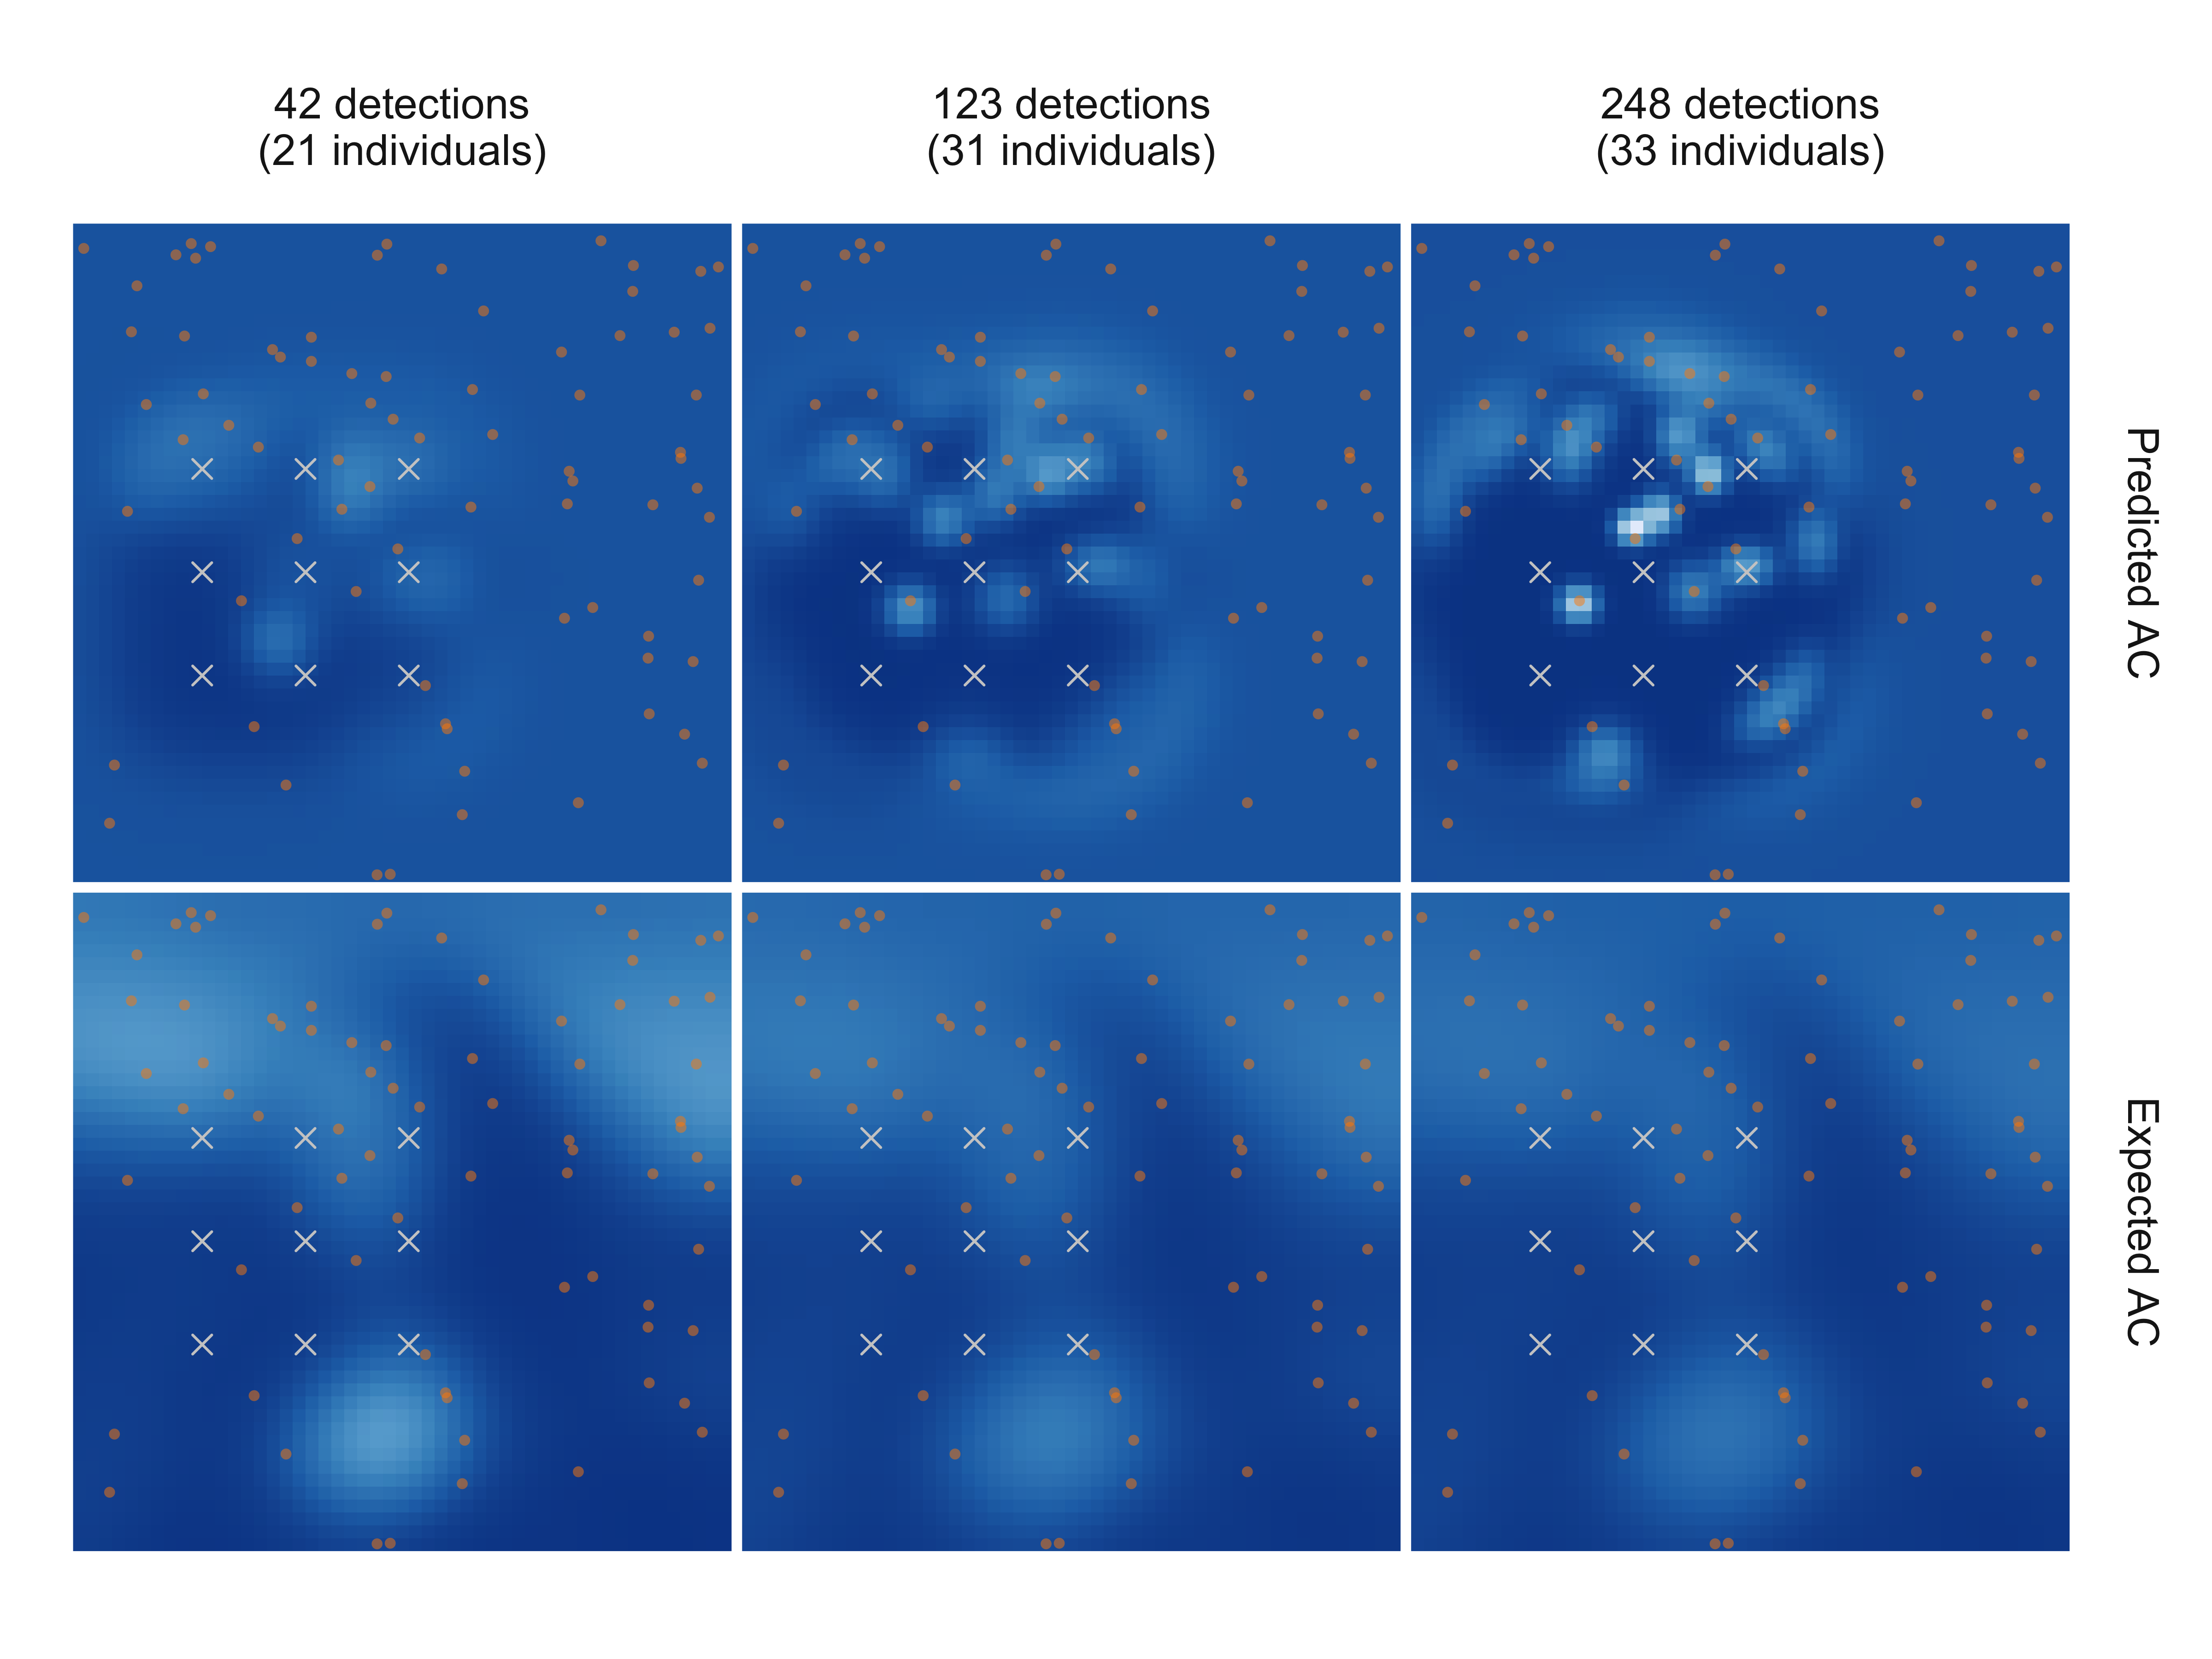
\includegraphics[width=1\textwidth]{mona_3x3.png}
\caption{Plots (a), (b), (c) show estimated realized AC surfaces estimated using the 3$\times$3 array indicated by grey crosses under three levels of survey effort. True AC locations are shown as orange dots. Plots (d), (e), (f) show expected activity center surfaces estimated using a model in which density is a function of a simulated spatially-varying covariate (see Figure \ref{mlinputs}c).}
\label{mona3x3}
\end{figure}


\begin{figure}[htbp]
\centering
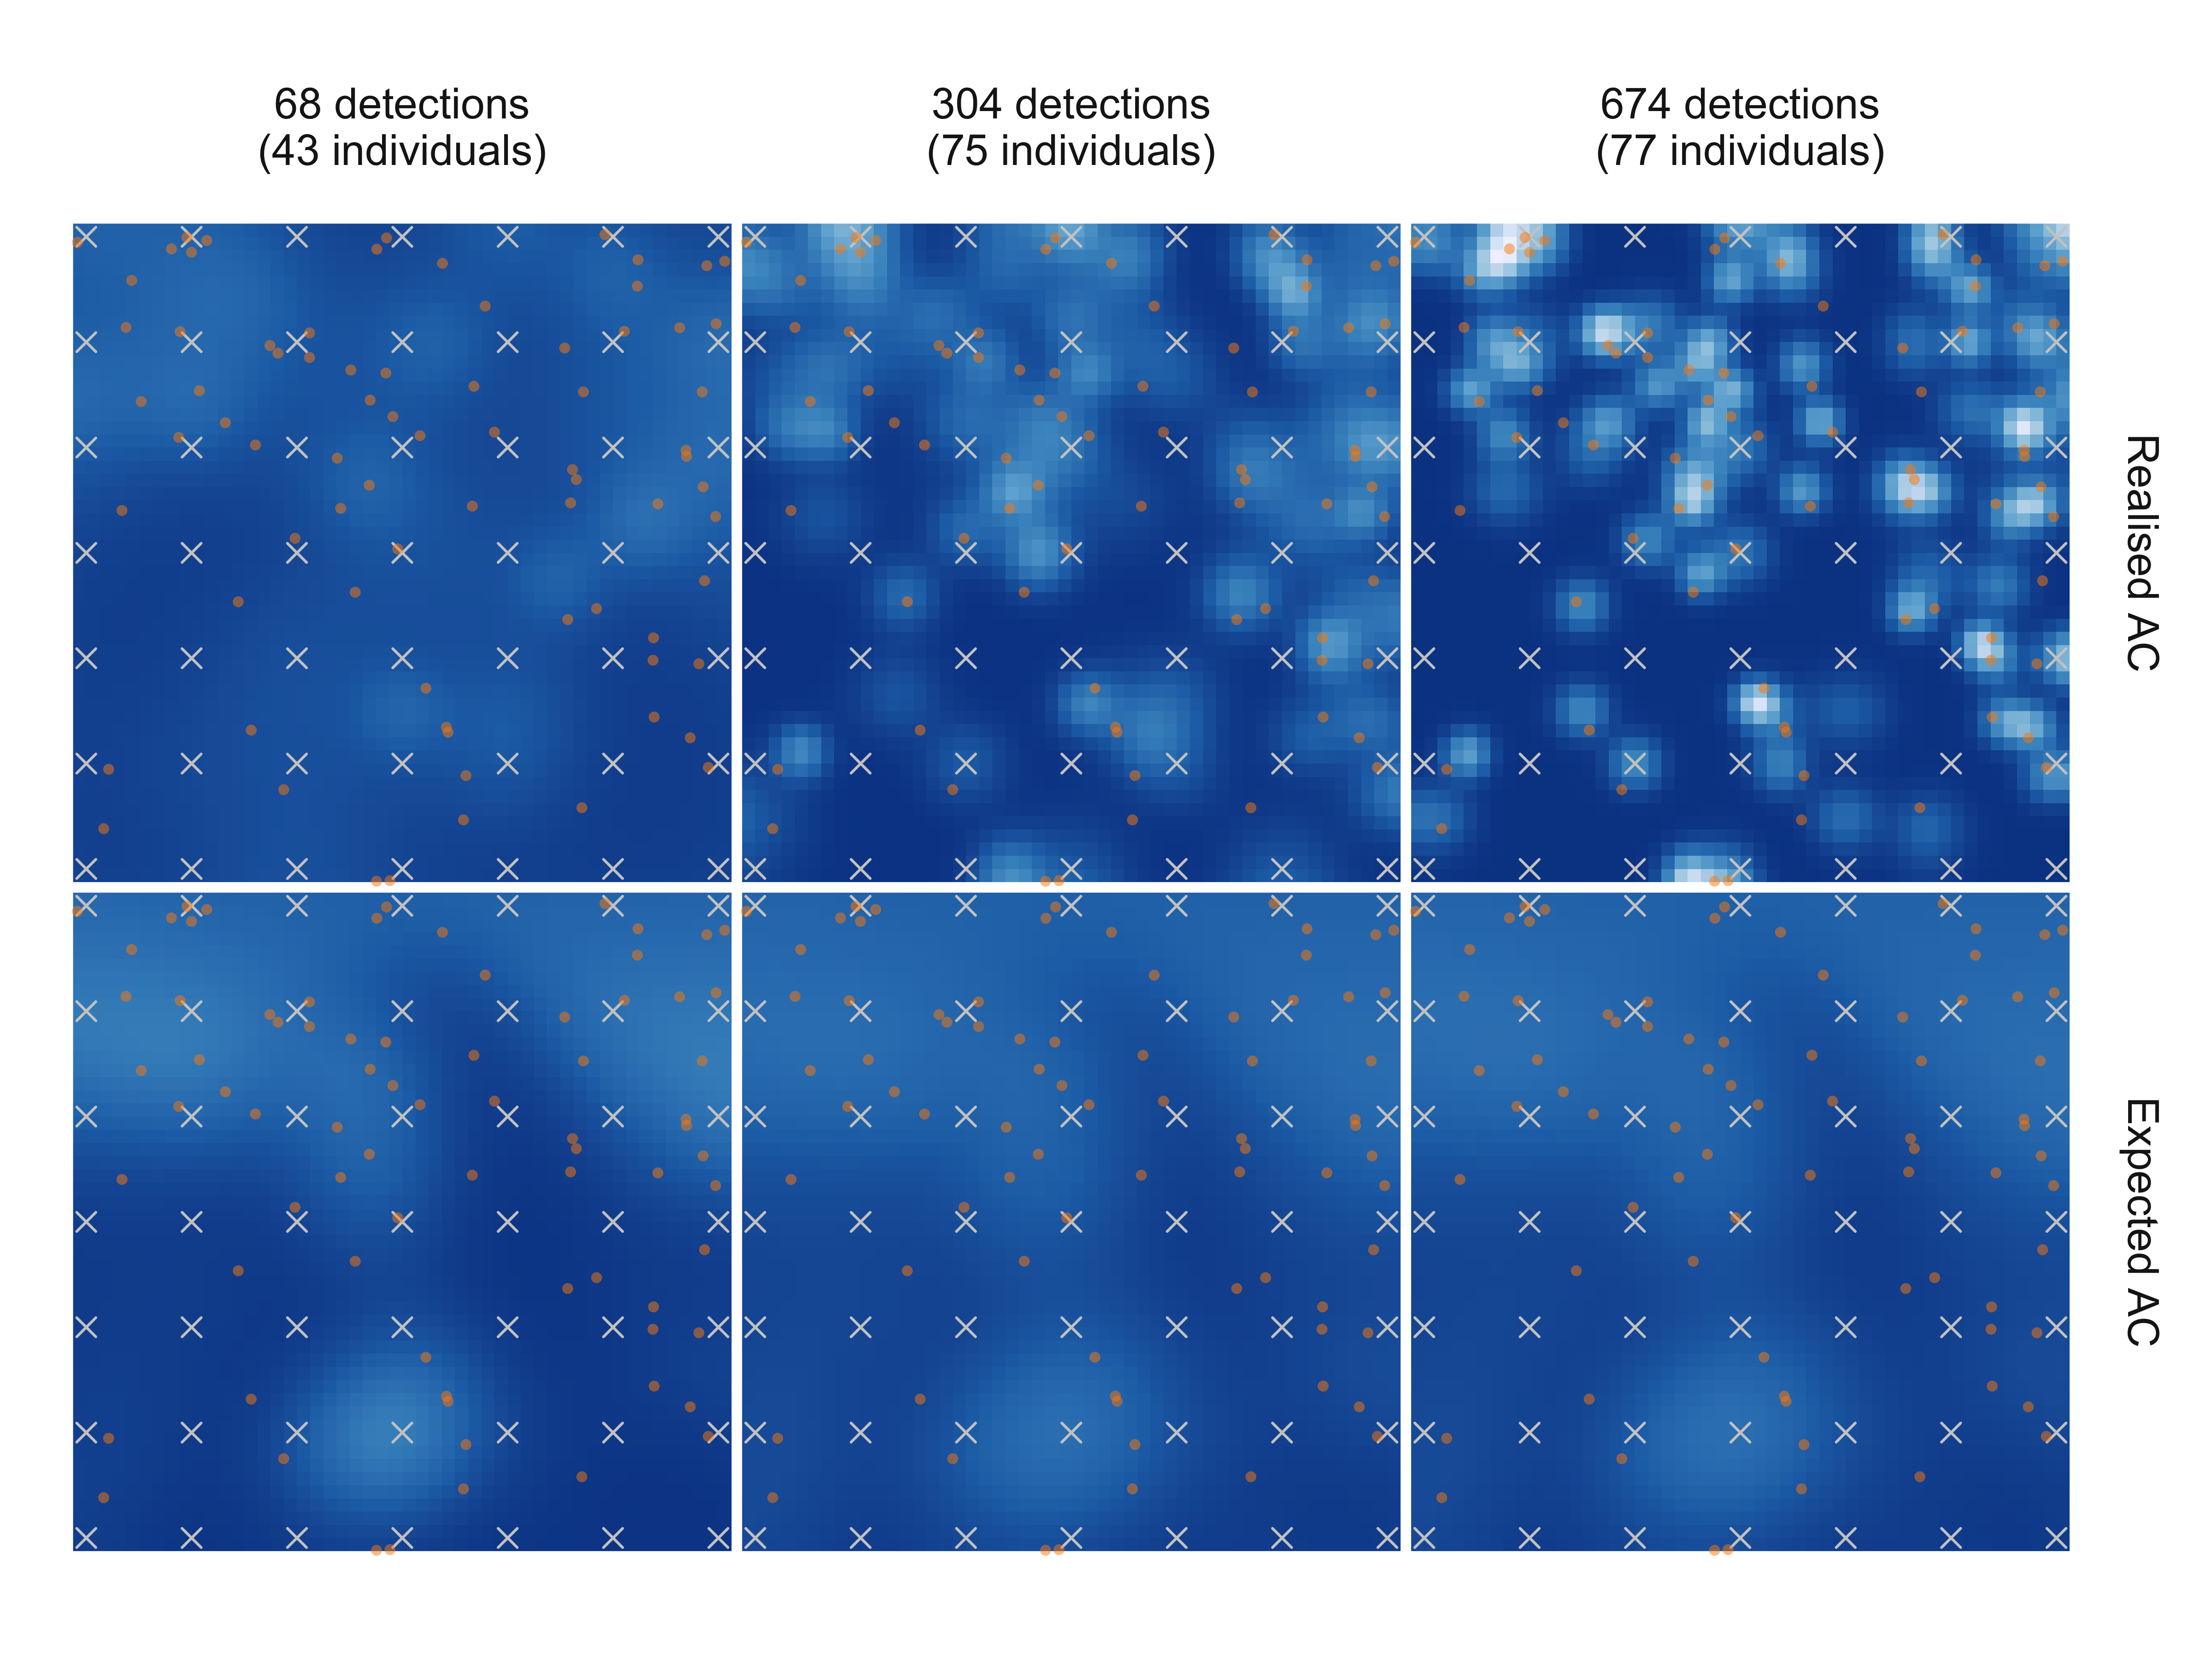
\includegraphics[width=1\textwidth]{mona_7x7.png}
\caption{Plots (a), (b), (c) show estimated realized AC surfaces estimated using the 7$\times$7 array indicated by grey crosses under three levels of survey effort. True AC locations are shown as orange dots. Plots (d), (e), (f) show expected activity center surfaces estimated using a model in which density is a function of a simulated spatially-varying covariate (see Figure \ref{mlinputs}c).}
\label{mona7x7}
\end{figure}

\section{Discussion and Conclusions} \label{discussion}
For most surveys, the realized AC density surfaces produced from an SCR model cannot be interpreted as density maps in any meaningful biological or ecological way, because they depend heavily on factors related to the detection process that have nothing to do with the underlying AC intensity. 

The surfaces will always show less spatial variability far from the detector array than close to, or within it, whether the underlying intensity is less variable there or not. This point is clearly stated in \cite{Royle+al:13a}, who say (pp.\ 165--166) ``As we move away from `where the data live' (away from the detector array) we see that the density approaches the mean density. This is a property of the estimator as long as the detection function decreases sufficiently rapidly as a function of distance. ... predictions tend toward the global mean as the influence of data diminishes'', and also in \textit{secr} documentation warning that ``There are serious problems with the interpretation of such plots as `density surfaces'... the surface depends on sampling intensity, and as more data are added it will change shape systematically. Ultimately, the surface near the centre of a detector array becomes a set of spikes on a barren plain'' \citep{secr:22}. A survey that uses greater survey effort will produce a realized AC density surface that has more spatial variability than a survey of exactly the same animals using lower effort. And the spatial variability moves with the array: move the array and the regions of high and low realized AC density move with it, even though the true ACs are unchanged.

A useful metaphor here might be of SCR as a torch shining a light onto the true activity centers -- what you see depends on where you shine the torch (detector locations) and how brightly you shine it (survey effort). If you interpret the uniform darkness outside of the beam to mean that everything outside the beam is the same, you fundamentally misunderstand the nature of torches and will draw fundamentally incorrect conclusions.

When considering realized ACs, SCR models answer the question ``where is an animal with {\it this} spatial capture history likely to have its activity center?'' The answer is always contingent on where detectors are located - because the capture history depends on where the detectors are located. This is the case regardless of whether one works in a Bayesian or frequentist framework. The same is true of the realized AC density surface, which simply sums estimated AC PDFs across animals, and will also be true for any downstream analyses that make use of realized AC densities e.g.\ density-weighted connectivity \citep{Morin2017}.

Uncertainty about the location of an animal's AC is affected by the number of times it is detected and the number of detectors it is detected at (and to some extent by the spatial configuration of those detectors). These quantities tend to be larger, and so uncertainty less, for animals whose ACs are within reach of more detectors. For a regularly spaced grid of detectors, this means that uncertainty is less for animals whose ACs are well inside the array than it is for animals whose ACs are near the border of the array. For irregularly spaced arrays (i.e.\ most surveys) systematic spatial differences in locational uncertainty exist within the array because sampling intensity is not uniform throughout the survey region -- detectors are more densely clustered in some subregions than others. Concerns about spatial differences in uncertainty are diminished when the surveyed area is large and surveyed with high and even detector intensity, and under these conditions the realized AC density surface provides a reasonable reflection of the spatial distribution of ACs, particuarly within the array. But these conditions are not likely to hold in most SCR studies.

To extend the metaphor, a torch beam's does not abruptly change from bright to dark. At the periphery of the beam (near the extent of the array) objects become increasingly difficult to see. Increasing the brightness of the torch makes everything within the beam easier to see, but also pushes back the periphery of the beam. Drawing a line at which the torch can no longer be trusted is to some extent arbitrary. 

An apparent way of enhancing the interpretability of realized AC density surfaces is to present accompanying surfaces that convey the uncertainty in the realized AC density estimate in each pixel. While measures quantifying the uncertainty in AC density surface estimates can be easily computed, we found that these were ineffective in communicating the systematic spatial differences in locational uncertainty that affect realized AC density surfaces (Supplementary Material B). Pixel-specific standard deviations were strongly correlated with the predicted density in that pixel, and so conveyed much the same pattern as the AC density surfaces. Coefficients of variation were highest in pixels with near-zero densities. Both of these measures indicated that uncertainty was highest within the array. In addition uncertainty in realized AC density surface estimates was sensitive to the arbitrary choice of grid cell size, with higher precision (lower standard deviations, for example) obtained with larger cell sizes. 

There is a way of using SCR so that parameter estimates can be interpreted in a biologically or ecologically meaningful way, and this is by modeling the intensity of the underlying process as a function of environmental covariates. Covariates allow one to see beyond the spatial extent of the array (see bottom rows of Figures~\ref{mona3x3} and \ref{mona7x7}), provided that the relationship between covariate and response is a good one, and that detectors cover a sufficient range of covariate values to estimate that relationship well. The resulting surfaces show the (estimated) intensity of the underlying process assumed to generate activity centers. These expected densities will be highest where environmental covariates are most favorable. Using covariate models, and associated model-based inference, is not without issues -- there is a danger of extrapolating the density surface beyond the range of covariates around the detectors, particularly with a log link function, and the relationship with density and covariate is assumed to be the same everywhere as it is around the detectors. Notwithstanding this, expected AC density surfaces are no longer strongly tied to one particular realization of the Poisson process or to where detectors are placed.

Ultimately, the appropriate density surface to use depends on the aims of the researcher. We have argued that the estimated realized AC density surface should not be used, because of the strong dependence on detector location and survey effort. But if the goal is to identify the ACs of {\it some} animals currently in the study region (and it does not matter which ones) then it may well be an efficient way of locating these, especially in the interior of large, evenly sampled survey regions. If the goal is to estimate where animals (not just the ones in the current realization) are likely to have activity centers, then the expected AC density surface, with density a function of covariates, should be used.

\section*{Acknowledgements}

This work was part-funded by the Royal Society of New Zealand through Marsden grant UOA-1929.

\bibliographystyle{biom}
\bibliography{monalisa}

\section*{Supporting Information}
Web Appendices and Figures referenced in Sections 3 and 5 are available with this paper at the Biometrics website on Wiley Online Library. All data and code used in the paper, along with model objects and results, are available at \url{https://github.com/david-borchers/monalisa}. If accepted we would use Zenodo to create a permanent DOI link to the version of the repository used to generate the results in the paper.

%\section*{Authors' contributions} 
%DB conceived the initial idea of clarifying density surface meanings. BS conceived the idea of usage density surfaces and developed the theory describing these. ID and RP designed the Mona Lisa simulations. ID and RP implemented the simulations using maximum likelihood methods. RC and BS implemented the simulations using Bayesian methods. ID designed and implemented the Nagarahole re-analysis. KS provided guidance on misinterpretation and feedback on proposed guidelines. DB, ID, BS and RC wrote the paper. All authors contributed critically to the drafts and gave final approval for publication.




\end{document}

